

\section{Введение}
\subsection{Цель работы}
Целью данной лабораторной работы является исследование и анализ характеристик чувствительности осциллографа, а также изучение фигур Лиссажу для разных отношений частот. В процессе работы будет выполнен расчет максимальной чувствительности, коэффициента усиления, а также проведены эксперименты для определения отклонений и их влияния на точность измерений.

\subsection{Решаемые задачи}
\begin{enumerate}
  \item Исследовать чувствительность пластин вертикального и горизонтального отклонений осциллографической трубки. 
  \item Наблюдать с помощью осциллографа синусоидальное напряжение, полученное с выхода генератора. 
  \item Получить фигуры Лиссажу и определить частоту исследуемого напряжения по фигурам Лиссажу.
\end{enumerate}

\section{Основная часть}

\subsection{Теоретическая часть}
Чувствительность горизонтальных и вертикальных пластин измеряется по формуле:
\begin{equation}
S = \frac{L}{2 \sqrt{2} \cdot U_{\text{eff}}}
\end{equation}
где \begin{itemize}
    \item \( S \) — чувствительность (мм/В),
    \item \( L \) — длина одного деления экрана осциллографа,
    \item \( U_{\text{eff}} \) — эффективное напряжение.
\end{itemize}


\subsection{Эксперимент}
Для получения термоэлектронной эмиссии катод трубки нагревают, подавая на нагреватель катода переменное напряжение. Вылетевшие из катода электроны ускоряются электрическим полем и движутся по направлению к аноду. По пути они пролетают через фокусирующий электрод, который собирает вылетевшие электроны в пучок, образуя электронный луч, который проходит между отклоняющими пластинами двух взаимно перпендикулярных плоских конденсаторов. Если в конденсаторах создать электрическое поле, то первый конденсатор С1 может отклонять луч в одном направлении, а второй конденсатор С2 – в перпендикулярном. Пройдя отклоняющие пластины конденсаторов, электронный луч попадает в широкую часть трубки. Экран электронно-лучевой трубки покрывается веществом, которое светится под действием электронного пучка. В результате на экране видно светящееся пятно F. При правильно подобранных напряжениях на катоде, аноде и фокусирующем электроде это пятно имеет размеры порядка 1 мм в диаметре.

\begin{figure}[ht!]
\centering
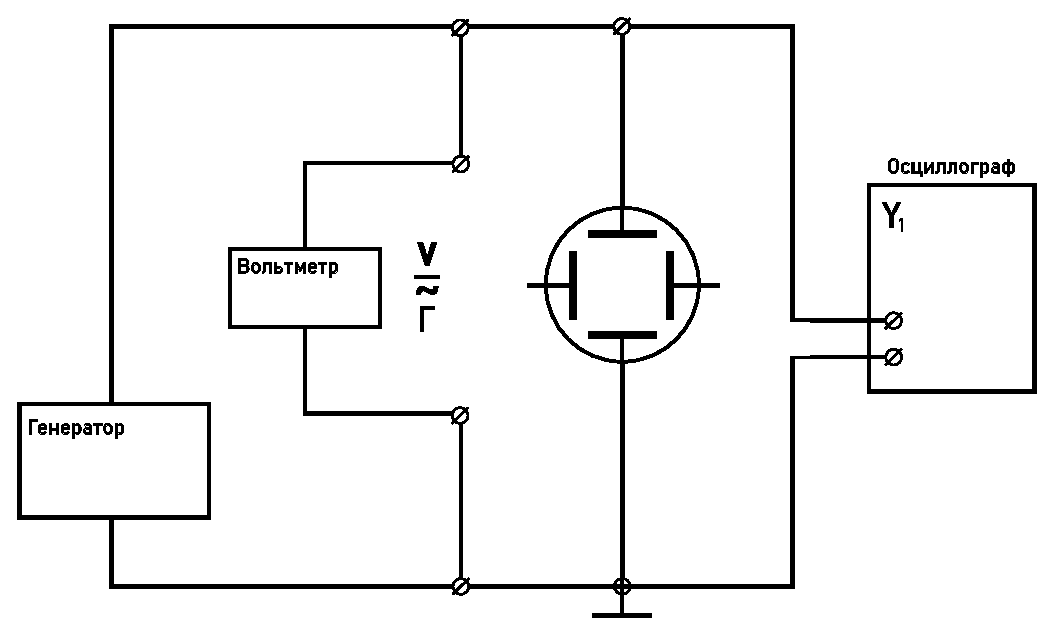
\includegraphics[width=0.8\textwidth]{схема_1.eps}
\caption{Схема установки}
\label{fig:sketch}
\end{figure}
\clearpage
\begin{figure}[ht!]
\centering
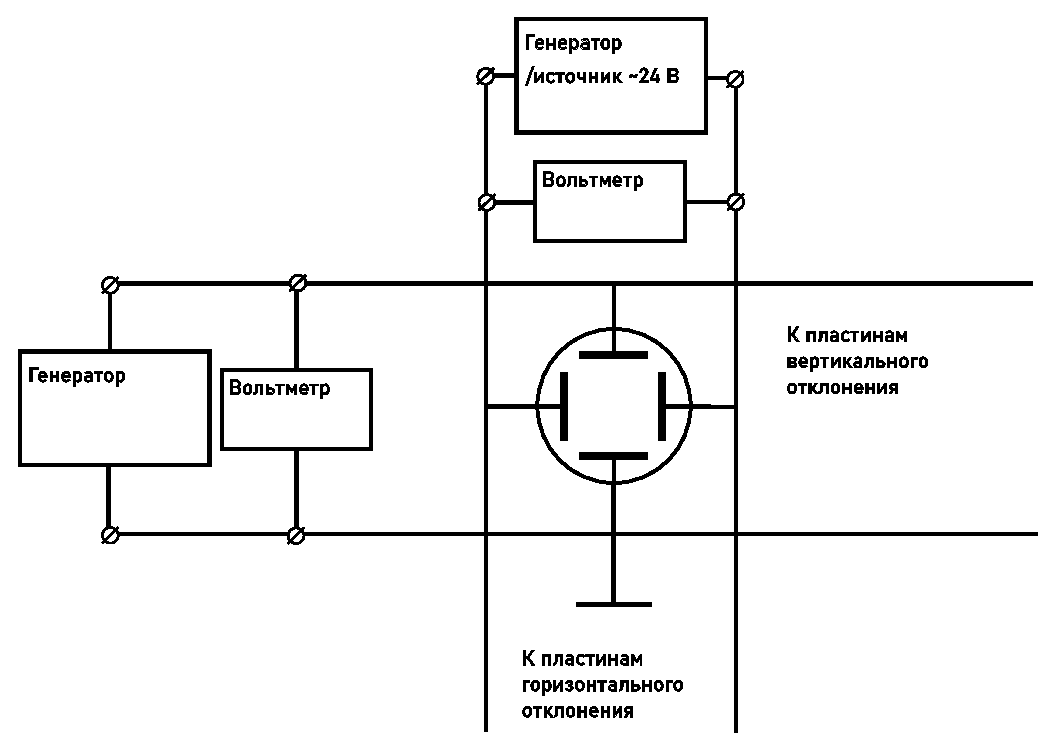
\includegraphics[width=0.8\textwidth]{схема_2.eps}
\caption{Схема установки}
\label{fig:sketch}
\end{figure}

\begin{figure}[ht!]
\centering
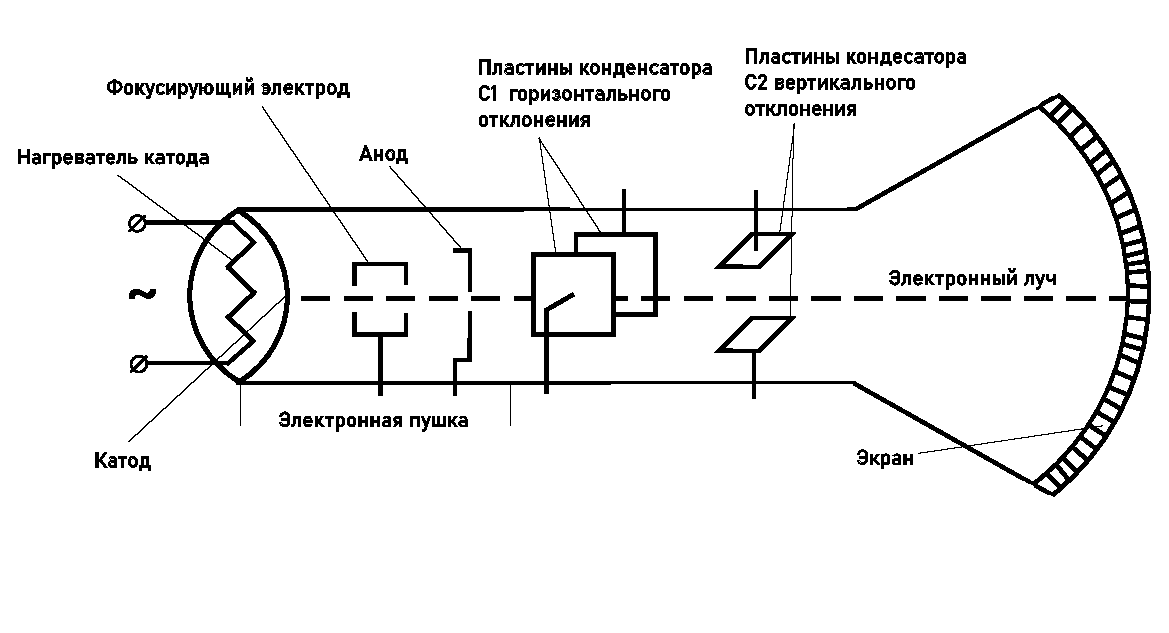
\includegraphics[width=0.8\textwidth]{схема_3.eps}
\caption{Схема установки}
\label{fig:sketch}
\end{figure}

\begin{figure}[H]
\centering
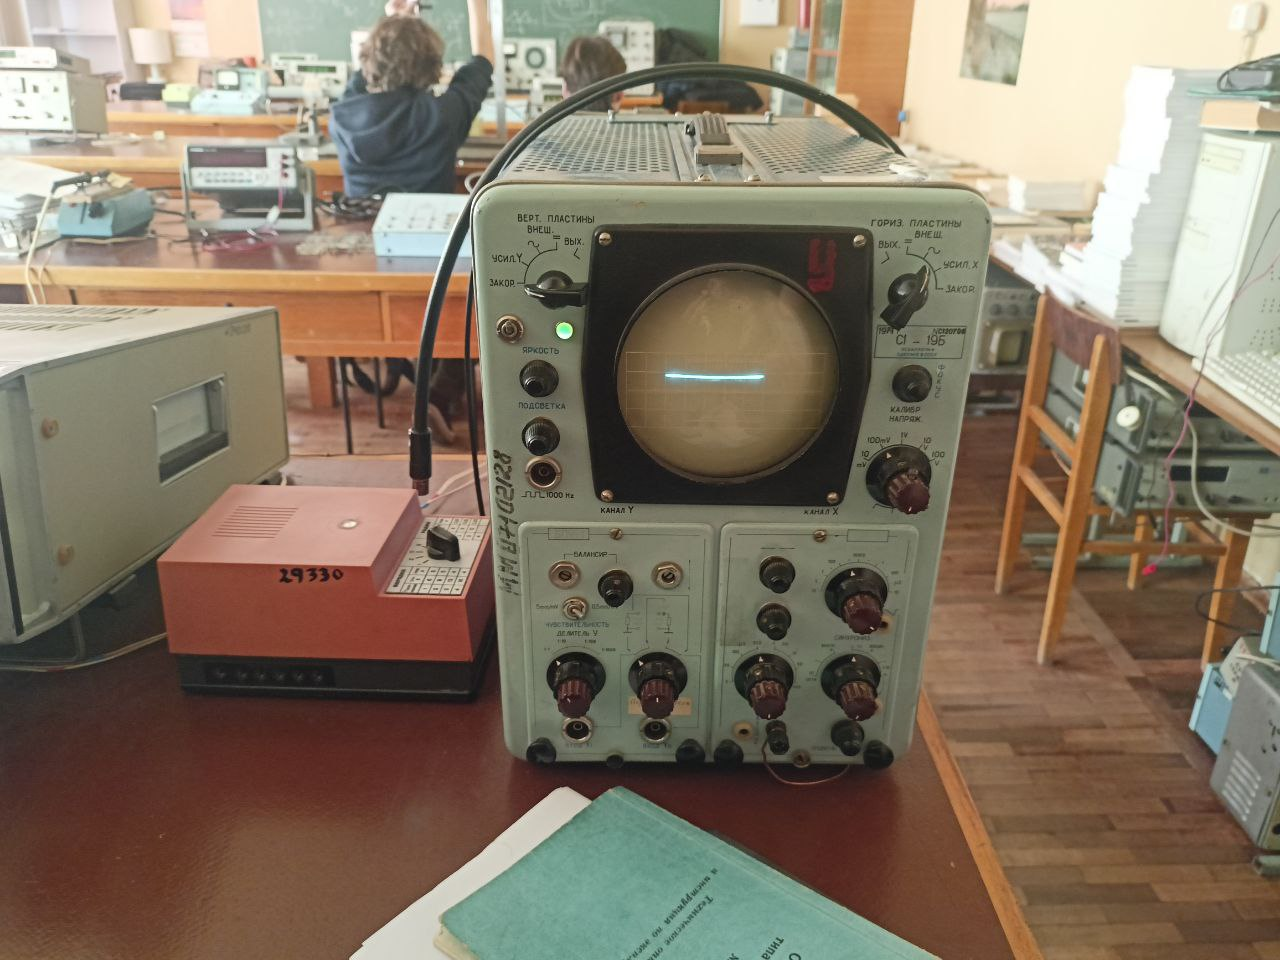
\includegraphics[width=0.6\textwidth]{1.jpg}
\caption{Фотография установки - осциллограф}
\label{fig:device}
\end{figure}

\begin{figure}[H]
\centering
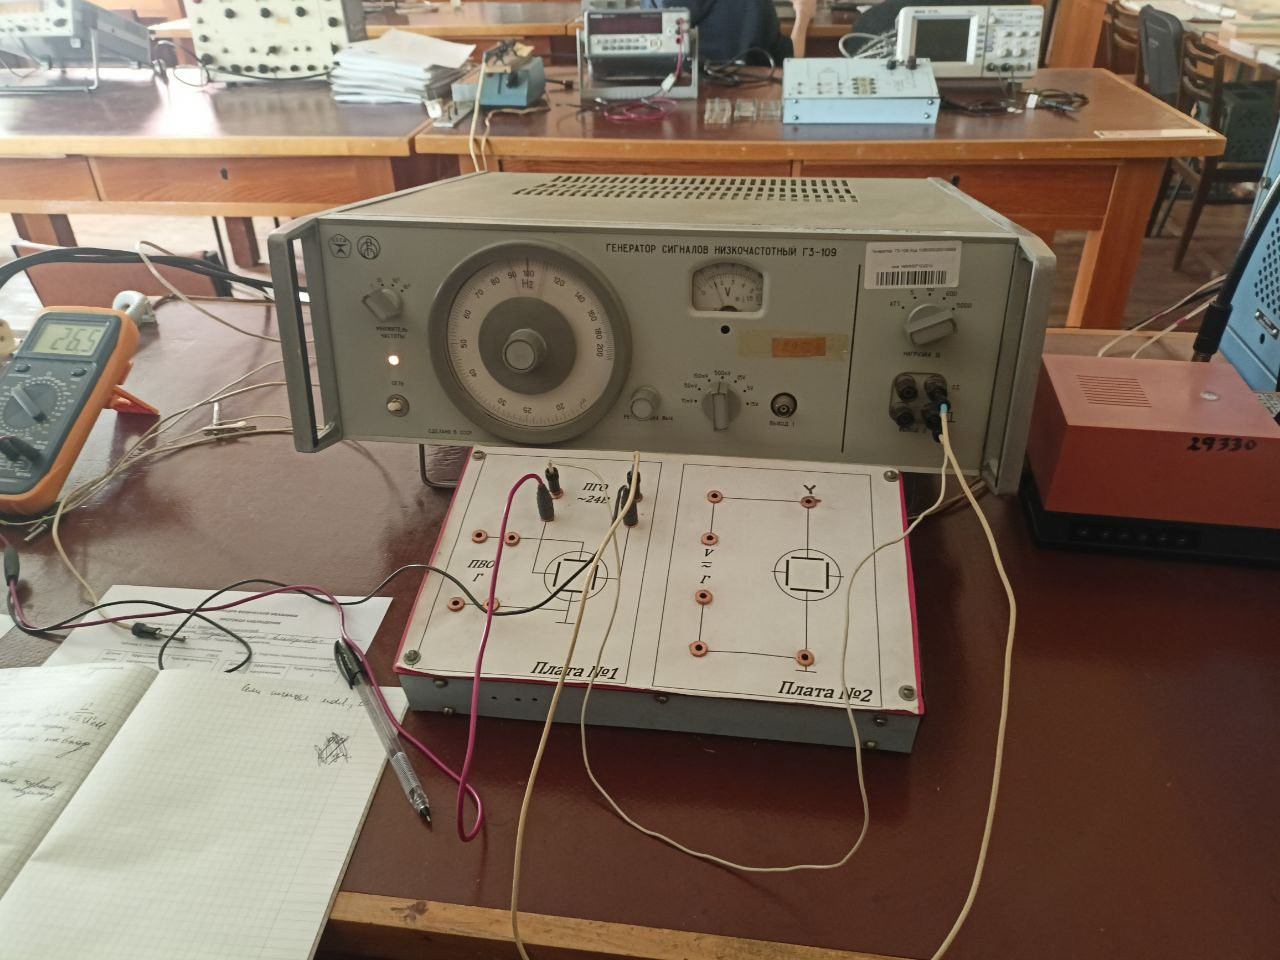
\includegraphics[width=0.6\textwidth]{2.jpg}
\caption{Фотография установки - генератор сигналов}
\label{fig:device}
\end{figure}


\subsection{Обработка данных и обсуждение результатов}

\subsubsection{Исходный код}
Для написания программы, вычисляющей все требуемые данные, используется язык C++; среда разработки - Visual Studio.

Данная программа на языке C++ предназначена для расчета чувствительности на основе данных, прочитанных из файлов.  Чувствительность вычисляется по формуле 
\[
    S = \frac{L}{2 \cdot \sqrt{2} \cdot U_{eff}}
\]
где (L) и (U) - входные данные, считываемые из текстовых файлов.  Программа обрабатывает три набора данных: вертикальные, горизонтальные и данные максимальных значений.  Результаты расчета чувствительности выводятся на экран и сохраняются в текстовый файл.
Программа выполняет следующие шаги:
\begin{enumerate}
    \item Чтение данных из текстовых файлов.
    \item Расчет чувствительности для каждого набора данных.
    \item Вывод результатов расчета чувствительности на экран.
    \item Запись результатов расчета чувствительности в файл.
\end{enumerate}

\begin{lstlisting}[label=listing1, caption=Функция считывания данных из файла]
std::vector<double> readData(const std::string& filename) {
    std::ifstream file(filename);
    if (!file.is_open()) {
        throw std::runtime_error("Не удалось открыть файл " + filename);
    }

    std::vector<double> data;
    double value;
    while (file >> value) {
        data.push_back(value);
    }

    return data;
}

\end{lstlisting}

\begin{lstlisting}[label=listing2, caption=Функция расчета чувствительности]
std::vector<double> calculateSensitivity(const std::vector<double>& L, const std::vector<double>& U)
{
	std::vector<double> sensitivity;

	for (size_t i = 0; i < L.size(); ++i)
	{
		double S = L[i] / (2 * std::sqrt(2) * U[i]);
		sensitivity.push_back(S);
	}

	return sensitivity;
}
\end{lstlisting}

\begin{lstlisting}[label=listing2, caption=Функция для вычисления среднего значения]
double computeAverage(const std::vector<double>& inputData) 
{
    double totalSum = 0.0;
    for (double num : inputData)
    {
        totalSum += num;
    }
    return totalSum / inputData.size();
}

// Функция расчета стандартного отклонения
double calculateStdDev(const std::vector<double>& dataVector) 
{
    double meanValue = computeAverage(dataVector);
    double squaredDiffsTotal = 0.0;

    for (double val : dataVector) {
        squaredDiffsTotal += std::pow(val - meanValue, 2);
    }

    return std::sqrt(squaredDiffsTotal / (dataVector.size() * (dataVector.size() - 1)));
}
\end{lstlisting}

\clearpage
\subsubsection{Таблицы}

\begin{center}
\begin{table}[h!]
\centering
\caption{Результаты наблюдений, расчет чувствительности для ПВО}
\label{tabl:1}
\begin{tabular}{|c|c|c|}
\hline
\begin{minipage}{5cm}
    Длина линии на экране, \( L \)
\end{minipage} &
\begin{minipage}{5cm}
    Эффективное напряжение, $U_{\text{eff}}$
\end{minipage} &
\begin{minipage}{5cm}
    Чувствительность, \( S \)
\end{minipage}\\
\hline
мм&В&мм/В\\
\hline
10 & 4,5 & 0.785674 \\
20 & 10,9 & 0,648722 \\
30 & 17,5 & 0,606092 \\
40 & 23,5 & 0,601793 \\
50 & 31,6 & 0,55942 \\
\hline
\end{tabular}
\end{table}
\end{center}

\begin{center}
\begin{table}[h!]
\centering
\caption{Результаты наблюдений, расчет чувствительности для ПГО}
\label{tabl:2}
\begin{tabular}{|c|c|c|}
\hline
\begin{minipage}{5cm}
    Длина линии на экране, \( L \)
\end{minipage} &
\begin{minipage}{5cm}
    Эффективное напряжение, $U_{\text{eff}}$
\end{minipage} &
\begin{minipage}{5cm}
    Чувствительность, \( S \)
\end{minipage}\\
\hline
мм&В&мм/В\\
\hline
10 & 3 & 1.17851 \\
20 & 8,5 & 0.83189 \\
30 & 13,7 & 0.774205 \\
40 & 20,2 & 0.700106 \\
50 & 26,5 & 0,667082 \\
\hline
\end{tabular}
\end{table}
\end{center}

\begin{center}
\begin{table}[h!]
\centering
\caption{Максимальная чувствительность осциллографа}
\label{tabl:3}
\begin{tabular}{|c|c|c|}
\hline
\begin{minipage}{5cm}
    Длина линии на экране, \( L \)
\end{minipage} &
\begin{minipage}{5cm}
    Эффективное напряжение, $U_{\text{eff}}$
\end{minipage} &
\begin{minipage}{5cm}
    Чувствительность, \( S \)
\end{minipage}\\
\hline
мм&В&мм/В\\
\hline
10 & 0,073 & 48.432 \\
20 & 0,12 & 58.9256 \\
30 & 0,196 & 54.1153 \\
40 & 0,351 & 40.291 \\
\hline
\end{tabular}
\end{table}
\end{center}

\begin{table}[h!]
\centering
\label{tabl:4}
\caption{Таблица исследования фигур Лиссажу}
\begin{tabular}{|c|c|c|c|c|}
\hline
Вид фигуры Лиссажу & o & 8 & ooo & oo \\
\hline
Отношение частот \( f_x/f_y \) & 1:1 & 2:1 & 1:3 & 1:2 \\
\hline
Частота по лимбу генератора \( f_y \), Гц & 50 & 25 & 150 & 100 \\
\hline
Исследуемая частота \( f_x \), Гц & 50 & 50 & 50 & 50 \\
\hline
\end{tabular}
\end{table}

\subsubsection{Графики}


Исходя из графиков ПВО и ПГО, можно заключить, что в диапазонах 10,9 – 31,6 (ПВО) и 8,5 – 26,5 (ПГО) приборы демонстрируют стабильную чувствительность. Для более точной оценки значений в этих зонах рассчитаем среднее арифметическое значение по трем соответствующим измерениям, а погрешность определим как стандартную ошибку этого среднего.

\[
S_y = 0.64034\, \text{мм/В}
\]
\[
S_x = 0.830359 \, \text{мм/В}
\]
\[
\Delta S = \sqrt{\frac{\sum_{i=1}^{n} (S_i - \overline{S})^2}{n(n-1)}}
\]

Таким образом:
\[
\Delta S_y = 0.0389866 \, \text{мм/В}, \quad \Delta S_x = 0.0916488 \, \text{мм/В}
\]

Максимальный коэффициент усиления:

\[
K_{\text{max}} = \frac{S}{S_y} = 92.022
\]
\clearpage
\begin{figure}[ht!]
\centering
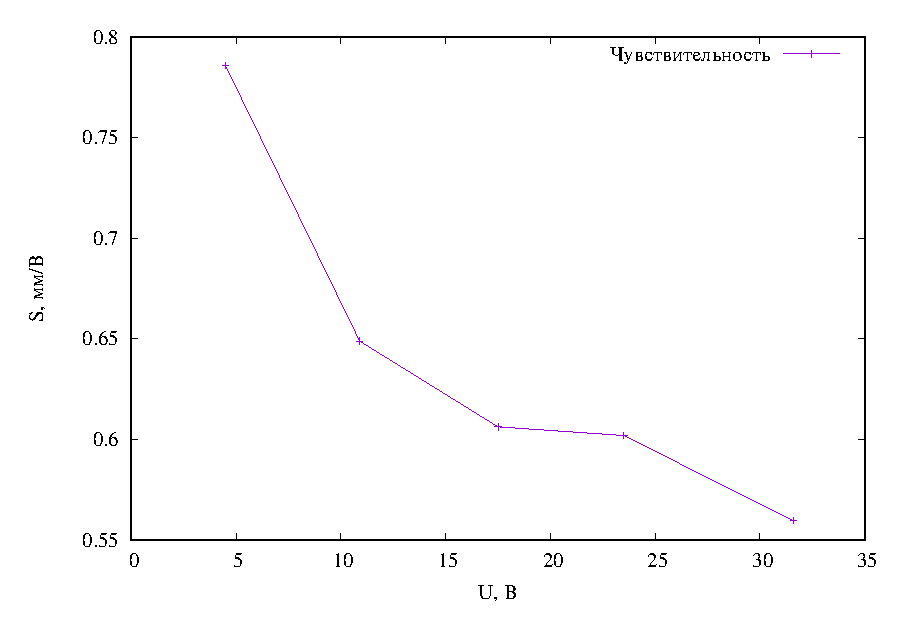
\includegraphics[width=0.8\textwidth]{sensitivity_vs_voltage.eps}
\caption{Зависимость чувствительности пластин вертикального отклонения от напряжения}
\label{fig:plot}
\end{figure}

\begin{figure}[ht!]
\centering
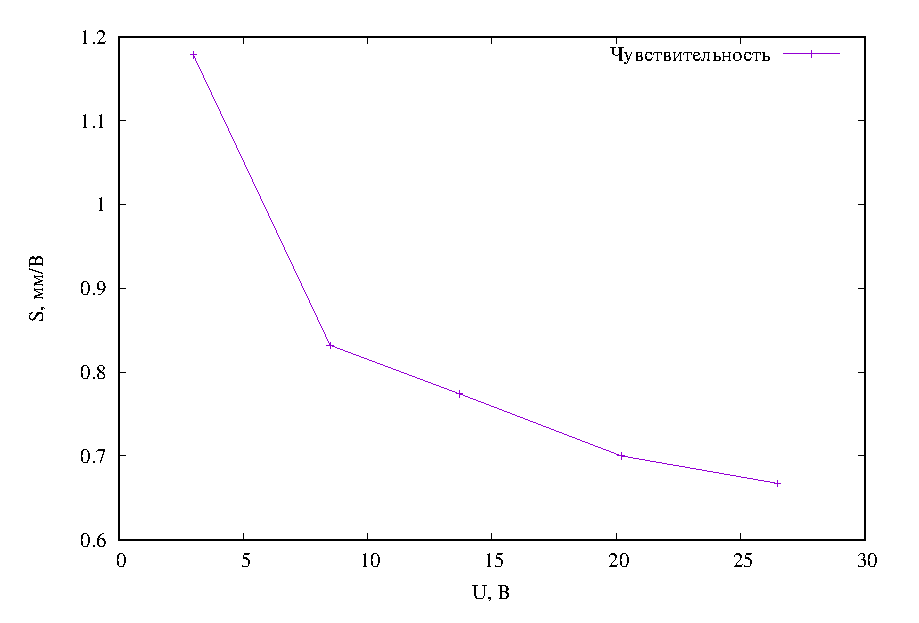
\includegraphics[width=0.8\textwidth]{sensitivity_vs_voltage_H.eps}
\caption{Зависимость чувствительности пластин горизонтального отклонения от напряжения}
\label{fig:plot}
\end{figure}

\section{Вывод}
 С использованием синусоидального напряжения на экране осциллографа были получены стационарные фигуры Лиссажу. Чувствительность вертикальных и горизонтальных отклоняющих пластин осциллографа была определена с помощью фигур Лиссажу. Частота исследуемого напряжения, вычисленная на основе этих фигур, составила 50 ± 0,5 Гц.

\begin{thebibliography}{9}

%ссылка на репозиторий с исходныим кодом отчета и всех расчетных программ обязательна 
\bibitem{repo}
\url{https://github.com/st117210/Workshop1.git}  


\end{thebibliography}
\clearpage
\appendix